\chapter{Neighbourhood component analysis}
\label{ch:nca}
	This chapter can be regarded as a self-contained tutorial on neighbourhood component analysis (NCA; \citealp{goldberger2004}). Much of the material is especially useful for the reader interested in applying the algorithm in practice. We start with a review of the NCA method (section \ref{sec:general-presentation}). Next we recast the NCA model into a class conditional kernel density estimation problem (section \ref{sec:cc-kde}). This new formulation will prove useful later when we want to alter the model in a principled way (section \ref{sec:nca-cs-back}). Lastly, in section \ref{sec:practical-notes} we present the learnt lessons from our experience with NCA. Both section \ref{sec:cc-kde} and \ref{sec:practical-notes} offer new insights into the NCA method and they also bring together related ideas from previous work.

\section{General presentation}
\label{sec:general-presentation}
	Neighbourhood component analysis learns a Mahalanobis metric that improves the performance of $k$ nearest neighbours ($k$NN). From a practical point of view, NCA  is regarded as a desirable additional step before doing classification with $k$NN. It improves the classification accuracy and it is also provides good low-dimensional representation of the data.

	Because the goal is to enhance the $k$NN performance, the first idea \citet{goldberger2004}
	had was to maximize the leave one out cross validation performance with respect to a linear projection~$\AB$. The procedure can be described as follows: apply the linear transformation~$\AB$ to the whole data set, then take each 
	point~$\AB\xB_i$ and classify it using $k$NN on the transformed data set~$\{\AB\xB_j\}_{j=1}^N$. The matrix~$\AB$ that achieves the highest number of correct classifications will be used for testing. However, finding the optimal $\AB$ is not easy. Any objective function based on the $k$ nearest neighbours
	is piecewise constant and discontinuous and, hence, hard to optimize. The reason is that there does
	not exist an exact correlation between $\AB$ and the neighbours
	of a given point: a small perturbation in $\AB$ might cause strong changes or, conversely, 
	it might leave the neighbours unchanged.
	
	The authors' solution lies in the concept of \textit{stochastic} nearest
	neighbours. Remember that in the classical $1$NN scenario, a query point gets the label of the closest point. In the stochastic nearest neighbour 
	case, the query point inherits the label of a neighbour with a probability that is inverse proportional with the distance. The stochastic function is reminiscent of the generalized logistic function or of the softmax activation used for neural networks. Let $p_{ij}$ denote the probability that the point~$j$ is selected as the nearest neighbour of the point~$i$. The value of $p_{ij}$ is given by:
	\begin{align}
		p_{ij} = \frac{
						\exp(-d_{ij}^2)
					  }{
						\sum_{\substack{k=1 \\k\neq i}}^N\exp(-d_{ik}^2)
					  },
	\label{eq:stochastic-neighbour}
	\end{align} where $d_{ij}$ represents the distance between point~$i$ and point~$j$ in the projected space, i.e. $d_{ij} = d(\AB\xB_i;\AB\xB_j) = (\xB_i-\xB_j)\tr\AB\tr\AB(\xB_i-\xB_j)$. Also we have to set $p_{ii}=0$: point~$i$ cannot pick itself as the nearest neighbour since we assume its label is not known.
	
	Now we can construct a continuous objective function using the stochastic assignments~$p_{ij}$ which are differentiable with respect to~$\AB$. A suitable quantity to optimize is the probability of each point of getting correctly classified. Point~$i$ is correctly classified when it is selected by a point~$j$ that has the same label as~$i$:
	\begin{align}
		p_i = \sum_{j\in c_i} p_{ij}.
		\label{eq:nca-p-i}
	\end{align}
	
	The objective function considers each point in the data set and incorporates their probability of belonging to the true class:
	\begin{align}
		f(\AB) &= \sum_{i=1}^N p_i\notag\\
			   &= \sum_{i=1}^N \sum_{j\in c_i} \frac{
								\exp(-d_{ij}^2)
							  }{
								\sum_{k\neq i}\exp(-d_{ik}^2)
							  }.
	\label{eq:nca-obj}
	\end{align}
	The score given by the objective function can be interpreted as the expected number of the correctly classified points.
	
	To obtain the best linear projection~$\AB$, we maximise $f(\AB)$ using an iterative gradient based solver such as gradient ascent, conjugate gradients or delta-bar-delta (subsection \ref{subsec:optimization}). For these methods, we can use the analytical expression of the gradient. If we differentiate with respect to $\AB$, we obtain:
	\begin{align}
	  \frac{\partial f}{\partial	\AB}=2\AB\sum_{i=1}^{N}\left(p_i\sum_{k=1}^Np_{ik}\xB_{ik}\xB_{ik}^{\textrm{T}} -
	\sum_{j\in c_i}p_{ij}\xB_{ij}\xB_{ij}^{\textrm{T}} \right)\label{eq:nca-grad},
	\end{align}
	where $\xB_{ij} = \xB_i - \xB_j$. The interested reader can find the derivation in the appendix. 

	At test time, we use the learnt matrix~$\AB$ to transform the points before doing classification with $k$NN. Given a query point $\xB^*$, we assign it the label~$c_j$ of the closest point~$j$ in the projected space, where $j = \operatorname{argmin}_{i}d(\AB\xB^*,\AB\xB_i)$.

	\subsection*{Further remarks}
	
	There are some interesting observations that can be made about NCA. It is useful to note that NCA model is still valid even if we set the matrix $\AB$ to be rectangular, i.e. $\AB\in\mathbb{R}^{d\times D}$, with $d<D$. In this case the linear transformation $\AB$ is equivalent to a low dimensional projection. Restricting $\AB$ to be non-square gives rise to a couple of advantages. Firstly, the optimization process is less prone to overfitting since a rectangular matrix has fewer parameters than a square one. Secondly, the low dimensional representation of the data set reduces the memory requirements and the computational cost at test time. In this thesis we concentrate mostly on low-rank metrics partly motivated by the above reasons, but also because many techniques that are subsequently developed (chapter \ref{ch:reducing}) work best in low dimensions.

	%equations \eqref{eq:stochastic-neighbour} to \eqref{eq:nca-grad} are still valid, since the distances $d_{ij}$ correspond to distances between points in a low dimensional space.

	We need to underline that NCA's objective function is not convex. The first consequence is that the parameter space is peppered with local optima and care must be taken to avoid poor solutions. Factors such as the choice of initialization or the optimization procedure affect the quality of the final result. Section \ref{sec:practical-notes} discusses these practical issues in detail. The other side of non-convexity is that it allows NCA to cope well with data sets that have multi-modal classes. This is an important advantage over classical methods such as principal component analysis, linear discriminant analysis or relevant component analysis. All of these assume that the data is normally distributed which harms the classification performance on complicated data sets.
% property has its advantage. It allows NCA to get good results on more complicated data sets that are not non convex. 

	Another important characteristic of NCA is its computational cost. For each point, we need to calculate the distances to all the other points. So the number of operations is quadratic in the number of data points. The evaluation of the objective function is done in two steps. First we find the point projections $\{\AB\xB_i\}_{i=1}^N$; this operation has $\mathcal{O}(dDN)$ cost. Next we compute all the distances~$d_{ij}$ in the low dimensional space; this is done in $\mathcal{O}(dN^2)$ flops. The total cost is then $\mathcal{O}(dDN+dN^2)$. Another way of evaluating the function~$f$ is to parametrize it in terms of the Mahalanobis metric $\SB=\AB\tr\AB$. Then we can compute the distances in the $D$-dimensional space in $\mathcal{O}(DN^2)$ flops. This option is slower than the previous case for $d<D$ and $D\ll N$.

	Since the optimization is based on the gradient, we are also interested in its cost. The evaluation of gradient given in the original paper and in equation~\eqref{eq:nca-grad} scales in $D^2N^2$. We improve this by ``pushing'' the matrix $\AB$ into the sum as in \citep{singh2010}:
	\begin{align}
	  \frac{\partial f}{\partial	\AB}=2\sum_{i=1}^{N}\left(p_i\sum_{k=1}^Np_{ik}(\AB\xB_{ik})\xB_{ik}^{\textrm{T}} -
	\sum_{j\in c_i}p_{ij}(\AB\xB_{ij})\xB_{ij}^{\textrm{T}} \right)\label{eq:nca-grad-alt},
	\end{align}

	If we consider that the projections $\AB\xB_i$ were already calculated for the function evaluation, the gradient has a cost of $\mathcal{O}(dDN^2)$. However, in theory, evaluating the gradient should have the same complexity as evaluating the objective function. Automatic differentiation (AD; \citealp{rall1981}) is a technique that achieve this theoretical result. AD uses the chain rule to derivative the objective function and split the gradient into elementary functions that can be readily computed. So instead of evaluating the complicated analytical gradient, we work on a series of cheap operations. This method is very useful in practice and there exist libraries for this in most programming languages. In our implementation we used the analytical differentiation, because we were not aware of AD until recently.
	
	The computational drawback represents an important setback in applying NCA in practice. For example, \citet{weinberger2007} reported that the method ran out of memory on large data sets and \citet{weizman2007} used only 10\% of an hyper-spectral data set to train the NCA classifier. We present a number of solutions to this problem in chapter \ref{ch:reducing}. 
	
% 	The general scenario in which NCA is applied can be described by the training and testing steps:
% 	describe algorithm.
	%\begin{itemize}
	%   \item
	%\end{itemize}
	
\section{Class-conditional kernel density estimation interpretation}
\label{sec:cc-kde}
	
	\begin{figure}
	  \centering
	  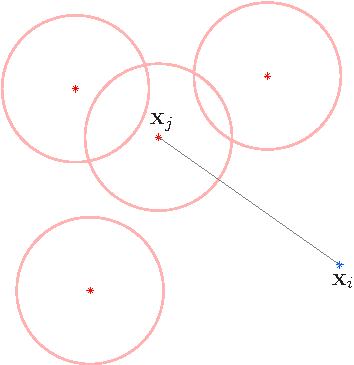
\includegraphics[width=6cm]{images/mog}
	  \caption{NCA as a class-conditional kernel density estimation
	model. The figure represents a schematic illustration of a mixture of Gaussians. The red circles denote isotropic Gaussians. These are centred onto the points that belong to a certain class. A point~$i$ is generated by either of the components of the class with a probability inverse proportional with the distance.}
	  \label{fig:kde}
	\end{figure}
	
	In this section we recast NCA into a class-conditional kernel density
	estimation framework. This interpretation will allow us to understand the assumptions behind NCA method. After this we are in position to alter the model in a suitable way that is efficient for computations (sections \ref{sec:approximate} and \ref{sec:exact-computations}).
	Similar ideas were previously presented by \citet{weinberger2007} and \citet{singh2010}, but the following were derived
	independently and they offer different insights. Our following interpretation
	was inspired by the probabilistic $k$NN presented by \citet{barber2011}.
	
	We start with the basic assumption that each class can be modelled by a mixture
	of Gaussians. For each of the $N_c$ data points in class $c$ we consider a
	Gaussian ``bump'' centred around it (figure \ref{fig:kde}). From a generative perspective, we can imagine
	that each point~$j$ can generate a point~$i$ with a probability given by
	an isotropic normal distribution with variance~$\sigma^2$:
	\begin{align}
	    p(\xB_i|\xB_j) &= \mathcal{N}(\xB_i|\xB_j, \sigma^2\mathrm{I}_D) \\
	                   &= \frac{1}{(2\pi)^{D/2}\sigma^D}\exp \left\{-\frac{1}{2\sigma^2}
	(\xB_i - \xB_j)^\mathrm{T}(\xB_i - \xB_j)\right\}.
	\end{align}
	
	By changing the position of the points through a linear transformation $\AB$,
	the probability changes as follows:
	\begin{align}
	    p(\AB\xB_i|\AB\xB_j) \propto \exp \left\{-\frac{1}{2\sigma^2} (\xB_i -
	\xB_j)^\mathrm{T}\AB^\mathrm{T}\AB(\xB_i - \xB_j)\right\}.
	\end{align}
	
	We note that this is similar to the $p_{ij}$ from NCA. Both
	$p(\AB\xB_i|\AB\xB_j)$ and $p_{ij}$ are directly proportional with the same
	quantity.
	
	Using the mixture of Gaussians assumption, we have that the probability of a
	point of being generated by class $c$ is equal to the sum of all Gaussians in
	class~$c$:
	\begin{align}
	    p(\xB_i|c) &= \frac{1}{N_c}\sum_{\xB_j \in c} p(\xB_i|\xB_j)
		\label{eq:p-x-c}
		\\
	               &= \frac{1}{N_c}\sum_{\xB_j \in c} \mathcal{N}(\xB_i|\xB_j,
	\mathrm{I}_D).
	\end{align}
	
	However, we are interested in the inverse probability, given a point $\xB_i$
	what is the probability of $\xB_i$ belonging to class $c$. We obtain the
	expression for $p(c|\xB_i)$ using Bayes' theorem:
	\begin{align}
	    p(c|\xB_i) = \frac{p(\xB_i|c)p(c)}{p(c|\xB_i)} =
	\frac{p(\xB_i|c)p(c)}{\sum_{c} p(\xB_i|c)p(c)}.
	    \label{eq:nca-cc-kde-bayes}
	\end{align}
	
	Now if further consider the classes to be equal probable (which is a
	reasonable assumption if we have no a priori information) we arrive at result
	that resembles the expression of $p_i$ (equation~\eqref{eq:nca-p-i}):
	\begin{align}
	%   &p(c|\xB_i) = \frac{p(\xB_i|c)}{\sum_{c} p(\xB_i|c)}\\
	    p(c|\AB\xB_i) = \frac{
	                \frac{1}{N_c}\sum_{\xB_j \in
	c}\exp\left\{-\frac{1}{2\sigma^2}(\xB_i -
	\xB_j)^\mathrm{T}\AB^\mathrm{T}\AB(\xB_i - \xB_j)\right\}
	                }
	                {
	                \frac{1}{N_{c'}}\sum_{c'} \sum_{\xB_k \in
	c'}\exp\left\{-\frac{1}{2\sigma^2}(\xB_i -
	\xB_k)^\mathrm{T}\AB^\mathrm{T}\AB(\xB_i - \xB_k)\right\}
	                }
	\end{align}
	
	%In the numerator we have the sum of
	We are interested in predicting the correct class of the point~$i$. So we
	try to find that linear transformation~$\AB$ that maximises the class
	conditional probability of this point $p(c_i|\AB\xB_i)$ to its true class~$c_i$.
	\begin{align}
	    f(\AB) = \sum_i p(c_i|\AB\xB_i).
	    \label{eq:nca-cc-kde-obj}
	\end{align}.
	
	As in section \ref{sec:general-presentation}, we can optimize the function using the gradient information. The gradient is the following:
	\begin{align}
	    \frac{\partial f}{\partial \AB} =
	      \sum_i \left\{
	                \frac
	                {
	                    \frac{\partial p(\AB\xB_i|c)}{\partial \AB}p(c)
	                }
	                {
	                    \sum_c p(\xB_i|c)p(c)
	                }
	                - \underbrace{\frac{
	                    p(\AB\xB_i|c)p(c)
	                }{
	                    \sum_c p(\AB\xB_i|c)p(c)
	                }}_{p(c|\AB\xB_i)}
	                \frac{
	                    \sum_c \frac{\partial p(\AB\xB_i|c)}{\partial \AB}p(c)
	                }{
	                    \sum_c p(\AB\xB_i|c)p(c)
	                }
	             \right \}.
	    \label{eq:nca-cc-kde-grad}
	\end{align}

	The main advantage of the above formulation is that we can construct different models simply by modifying the class-conditional probability (equation~\eqref{eq:p-x-c}). Once $p(\xB_i|c)$ is altered in a suitable way, we use Bayes rule in conjuction equations~\eqref{eq:nca-cc-kde-obj} and~\eqref{eq:nca-cc-kde-grad} to get the new function and its corresponding gradient. We optimize for parameter $\AB$ exactly in the same way as for classical NCA.
	
	Examples of this technique are in sections \ref{sec:exact-computations} and \ref{sec:nca-cs-back}. There the alterations allowed considerable speed-ups as we shall see in chapter \ref{ch:evaluation}. 

	Other benefits of CC-KDE model are the possibility to incorporate prior information about the class distributions~$p(c)$ and the possibility to classify a point~$\xB^*$ using $p(c|\AB\xB^*)$ (subsection \ref{subsec:doing-classification}).

\section{Practical notes}
\label{sec:practical-notes}

	While NCA is not that hard to implement (appendix~\ref{app:code-nca-obj}), there is needed certain care
	in order to achieve good solutions.
	In this section we try to answer some of the questions 
	that can be raised when implementing NCA. 	

\subsection{Optimization methods}
\label{subsec:optimization}

	The function $f(\AB)$, equation~\eqref{eq:nca-obj}, can be maximised using any gradient based optimizer. We considered two popular approaches for our implementation: gradient ascent and conjugate gradients. These are only briefly presented here. The interested reader is pointed to \citep{bishop1995}.

	\subsubsection*{Gradient ascent}

	Gradient ascent is one of the simplest optimisation methods. It is an iterative algorithm that aims to find the maximum of a function by following the gradient direction at each step. The entire procedure is summarized by algorithm~\ref{alg:gd}. 

	Besides this version, an alternative is to compute the gradient on a fewer points and not on the entire data set. This variant is known as stochastic gradient ascent and it has the advantage to be much faster than the batch version. Different alterations of the stochastic gradient ascent were tried in chapter~\ref{ch:reducing} to reduce the computational cost.
      
	\begin{algorithm} 
		\caption{Gradient ascent (batch version)} 
		\label{alg:gd}  
		\begin{algorithmic}[1]                    % enter the algorithmic environment
			\REQUIRE Data set $\mathcal{D}=\{\xB_1,\cdots,\xB_N\}$.
			\STATE{ Get initial $\AB_0$ } \label{alg:gd-init}
			\REPEAT
				\STATE {Update parameter: $\AB_{t+1}\leftarrow \AB_{t} + \eta\frac{\partial
f(\AB_{t},\mathcal{D})}{\partial\AB}$}
				\STATE {Update learning rate $\eta$}
				\STATE {$t\leftarrow t+1$}
			\UNTIL {convergence}
			\RETURN $\AB_{t}$.
		\end{algorithmic}
	\end{algorithm}

	For the algorithm~\ref{alg:gd}, there are three aspects we need to carefully consider:
	\begin{description}
	 \item[Initialization.] The algorithm starts the search in the parameter space from the an initial parameter~$\AB_0$. Different values for $\AB_0$ will give different final solutions. In the NCA context, initialization is related to finding a good initial linear transformation; this is discussed  separately in subsection~\ref{subsec:initialization}. For the moment, we can assume the values of $\AB_0$ are randomly chosen.
	 \item[Learning rate.] The parameter $\eta$ is called \textit{step size} or, in neural networks related literature, it also known as \textit{learning rate}. As name suggests, $\eta$ controls how much we move the parameters in the gradient direction. 

	The learning rate can be either fixed or adaptive. For the first case, choosing the correct value for $\eta$ is critical. If $\eta$ is set too large, the algorithm diverges. On the other hand, a small $\eta$ results in slow convergence. 

	Usually, a variable learning rate $\eta$ is preferred since it is more flexible. The ``bold driver'' \citep{vogl1988} is a reasonable heuristic for automatically modifying $\eta$ during training. The idea is to gradually increase the learning rate after each iteration as long as the objective function keeps improving. Then we go back to the previous position and start decreasing the learning rate until a new increase in the function is found. The common way to increase the step size~$\eta$ is by multiplying it with a constant $\rho>1$, usually $\rho=1.1$. To decrease the step size, we can multiple it with a constant $\sigma<1$, for example $\sigma = 0.5$.
% This procedure is described in algorithm. The parameters indicate how much the learning rate is adjusted at each step. Usually, $\rho=1.1$ and $\sigma=0.5$.

% 	\begin{algorithm} 
% 		\caption{Gradient ascent with ``bold driver'' heuristic} 
% 		\label{alg:gd-bd}  
% 		\begin{algorithmic}[1]                    % enter the algorithmic environment
% 			\REQUIRE Data set $\mathcal{D}=\{\xB_1,\cdots,\xB_N\}$.
% 			\STATE{ Get initial $\AB_0$ } \label{alg:gd-init}
% 			\REPEAT
% 				\STATE {Update parameter: $\AB_{t+1}\leftarrow \AB_{t} + \eta\frac{\partial
% f(\AB_{t},\mathcal{D})}{\partial\AB}$}
% 				\STATE {Update learning rate $\eta$}
% 				\STATE {$t\leftarrow t+1$}
% 			\UNTIL {convergence}
% 			\RETURN $\AB_{t}$.
% 		\end{algorithmic}
% 	\end{algorithm}
	
	Another way is to change the learning rate~$\eta$ using a decreasing rule proportional to the number of current iteration: $\eta=\frac{\eta_0}{t+t_0}$. Now we have two parameters instead of one. Intuitively, $\eta_0$ can be regarded as the initial learning rate and $t_0$ as the number of iterations after which $\eta_0$ starts to drop off. Using a learning rate of such form is especially motivated in the stochastic gradient case. If $\eta\propto 1/t$, the algorithm converges to the true minimum as $t$ goes to infinity. However, in practice the convergence is very slow; so setting the constants~$\eta_0$ and~$t_0$ is important for reaching a good solution in a short time. Leon Bottou\footnote{Oral communication: \url{http://videolectures.net/mmdss07_bottou_lume/}} recommends to set $\eta_0$ to be the regularization value and then select $t_0$ such that the resulted update will modify $\AB$ with a sensible amount. Since we did not use regularization, we followed some of the tricks presented in \citep{lecun1998}. We fixed the value for $\eta_0$ and we did an exponential search for $t_0$ using a cross validation set. 

% 	A popular choice for an 
	 \item[Convergence.] The gradient ascent algorithm can be stopped either when we hit a maximum number of iterations or when the learning rate~$\eta$ falls below a certain threshold. Also we can look at the variation in the objective function. If the value of the objective function stops improving we can halt the algorithm. Another popular choice to check convergence is ``early stopping''. We monitor the performance of the new $\AB$ on a cross validation set. If the objective function did not increase for more than a preset number of iterations we stop and return to the previous best solution. This solution prevents overfitting since we stop when we achieve a minimum on a test error and not on the training error. We illustrate this in figure \ref{fig:early-stopping}.
	\end{description}
	
	\begin{figure}
	 \centering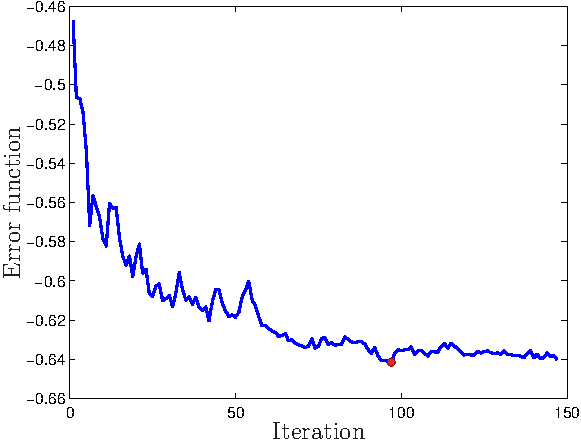
\includegraphics[width=0.59\textwidth]{images/early-stopping}
	 \caption{This figure illustrates the early stopping procedure. During training we keep a small part of the data set apart, for cross-validation. On this cross-validation data set we compute the error function at each iteration. When the error function stops decreasing we stop the learning procedure and return to the parameter that achieved the best value. This figure resulted while applying NCA on the \texttt{mnist} data set. The best value was obtained at iteration 98, as indicated by the red dot.}
	 \label{fig:early-stopping}
	\end{figure}


	Gradient ascent has known convergence problems and determining good learning rates is often difficult. But it has the advantage of being quite flexible, especially in the stochastic optimization scenario, where we can select any noisy estimate of the gradient in order to replace the total gradient.

	\subsubsection*{Conjugate gradients}
	
	Conjugate gradient (CG) method solves some of the convergence issues. Instead of selecting the search directions to be the gradient directions, CG method selects the next direction depending on both the previous directions and on the curvature of surface. This permits this method to reach the maximum of a quadratic energy function in only two iterations. Also CG eliminates the manual set-up for the learning rates. As \citet{bishop1995} notes, the CG can be regarded as a more complex version of gradient ascent that automatically chooses the parameters. The details of the conjugate gradient method are out of the scope of this thesis; a gentle introduction into the subject is given by \citet{shewchuk1994}.

	In practice it is considerably easier to  use an existing implementation of CG (for example, Carl E. Rasmussen's \texttt{minimize.m}\footnote{Source code can be found at the following URL: \url{http://www.gaussianprocess.org/gpml/code/matlab/util/minimize.m}}) than trying to find the optimal parameters for the learning rate for gradient ascent. For small and medium-sized data sets, ``bold driver'' heuristic gives comparable scores to the more fancier CG method (tables \ref{table:comp-opts-1} and \ref{table:comp-opts-2}).
	

% \begin{itemize}
%     \item We have the first-order gradient information; so, we
%         can use any gradient based method.
%     \item Gradient descent is an iterative algorithm that uses
%         first-order information to find a minimum of a
%         function. At each step, it proposes to go in the
%         steepest direction, \ie, the direction with largest
%         gradient. It is a very simple to implement method, but
%         suffers from known convergence drawbacks. For example,
%         there might appear the zig-zagging effect it depends
%         on some critical parameters which make it difficult to
%         use in practice. These are the learning rate $\eta$
%         and the convergence conditions.
%     \item Common choices for $\eta$ are either using a
%         constant step or decrease it gradually. Using a
%         constant step size can make the algorithm diverge.
%     \item There are different other heuristics that make this
%         more efficient. One of these is the bold-driver trick.
%     \item A learning rate decreasing procedure is to set
%         $\eta=\frac{\eta_0}{t + t_0}$, where $t$ represents
%         the iteration number, $\eta_0$ and $t_0$ are
%         constants. So, we end up with two hyper-parameters
%         instead of one. There are various trick of tuning
%         them. Leon Bottou mentions that a common value for
%         $\eta_0$ is to be equal to the regularization variable
%         and $t_0$ should then be selected such that the
%         updates . In our implementation, because we did not
%         use a regularization term, we set $\eta_0$ to a fix
%         value and then we did an exponential search for $t_0$.
%     \item One might also try to use momentum. For further
%         useful advice on optimization one should consult
%         BackProp.
%     \item An improved version of the gradient descent is the
%         conjugate gradients algorithm. This has better
%         convergence.
% \end{itemize}

\subsection{Initialization}
\label{subsec:initialization}

    \begin{figure}
	  \centering
	  \subfigure[Initial random projection]{\label{fig:init-1}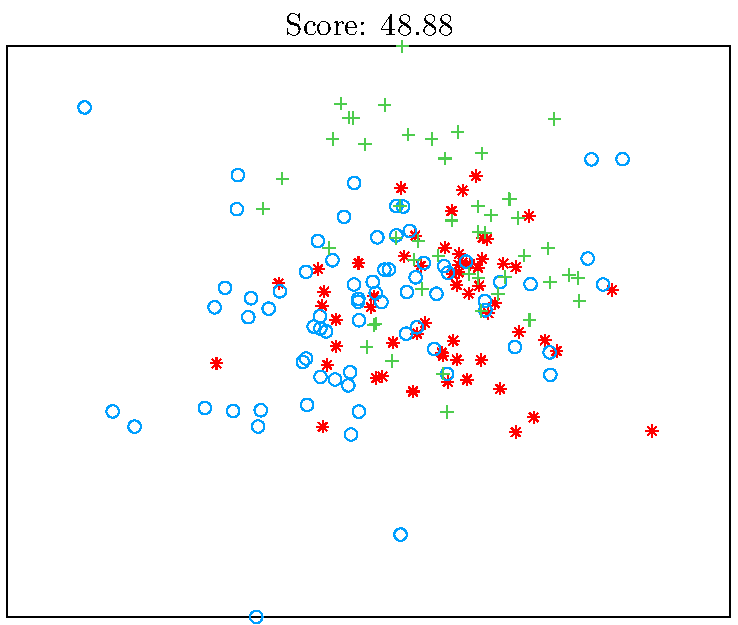
\includegraphics[width=0.49\textwidth]{images/wine-init-1}}
	  \subfigure[NCA projection after random initialization]{\label{fig:init-2}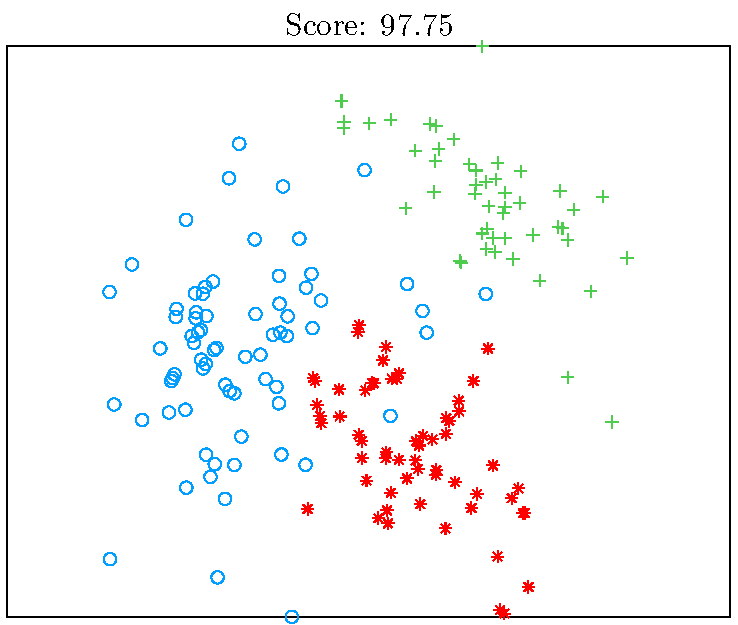
\includegraphics[width=0.49\textwidth]{images/wine-init-2}}

	  
	  \subfigure[Initial projection using PCA]{\label{fig:init-3}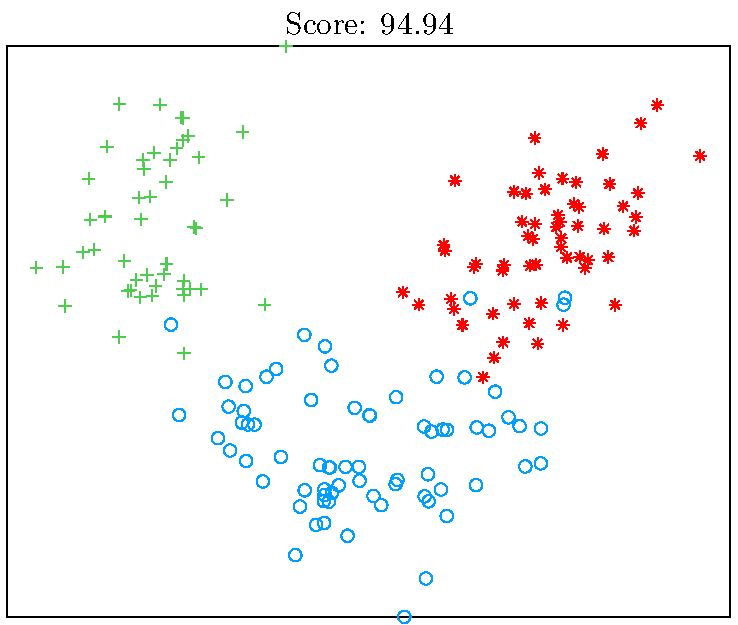
\includegraphics[width=0.49\textwidth]{images/wine-init-3}}
	  \subfigure[NCA projection after PCA initialization]{\label{fig:init-4}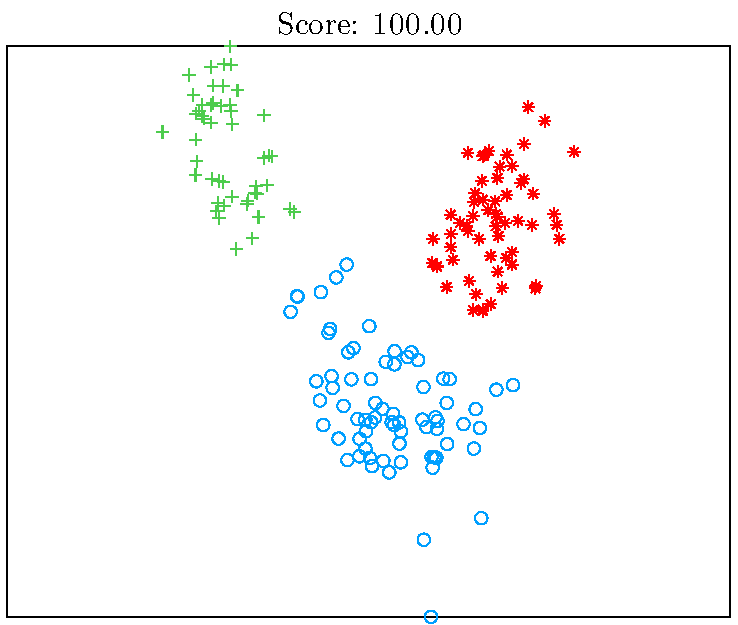
\includegraphics[width=0.49\textwidth]{images/wine-init-4}}

	  
	  \subfigure[Initial projection using LDA]{\label{fig:init-7}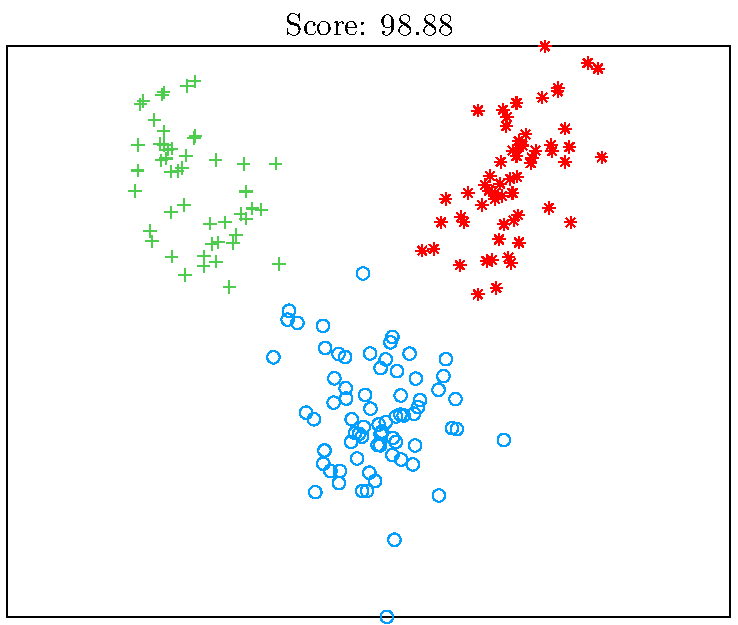
\includegraphics[width=0.49\textwidth]{images/wine-init-5}}
	  \subfigure[NCA projection after LDA initialization]{\label{fig:init-8}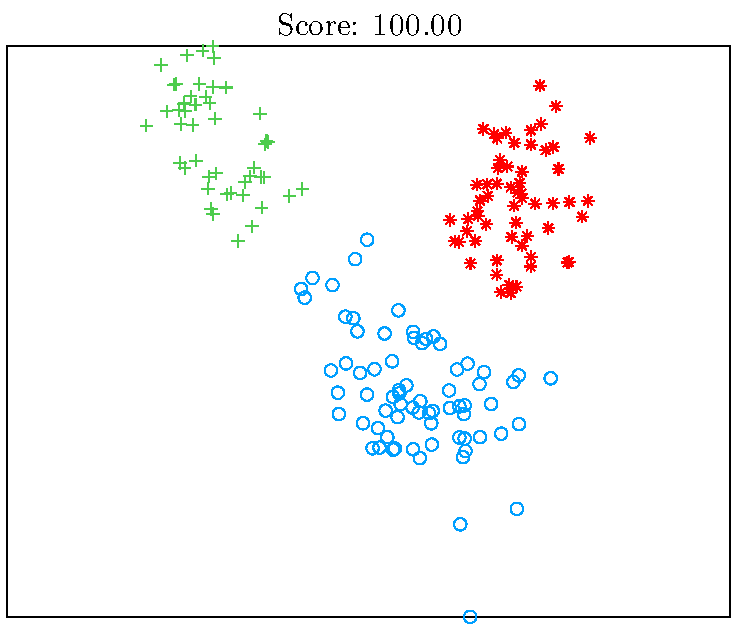
\includegraphics[width=0.49\textwidth]{images/wine-init-6}}
	  
	  \caption{\small Results for different initializations (random, PCA and LDA) on \texttt{wine} data set. The images on the left side represent the projections of the data set using the initial $\AB$. The images on the right side are data set projection with the final $\AB$. Above each figure there is presented the LOOCV score which is normalized to 100.}
	  \label{fig:init}
    \end{figure}

    Initialization is important because the function $f(\AB)$ is not convex. The quality of the final solution relies on the starting point of the optimisation algorithm. A general rule of thumb is to try multiple initial seeds and select that final $\AB$ that gives the highest score.

    We have already mentioned random initialization in subsection \ref{subsec:optimization}. Beside this, we can try linear transformations that are cheap to compute. Such examples include  principal component analysis (PCA; \citealp{pearson1901}), linear discriminant analysis (LDA; \citealp{fisher1936}) and relevant component analysis (RCA; \citealp{bar2003}). For completeness, we give here the equations and also include further notes:
        \begin{itemize}
            \item  PCA finds an orthogonal linear
                transformation of the data. This is
                obtained by computing the
                eigendecomposition of the outer covariance
                matrix:
                \begin{align}
                    \SB = \frac{1}{N}\sum_{i=1}^N (\xB-\muB)(\xB-\muB)\tr.
                    \label{eq:pca-1}
                \end{align}

            \item LDA finds a linear transformation $\AB$ by maximizing the
variance between classes $\SB_B$ relative to the amount of within-class variance
$\SB_W$:
            \begin{align}
             \SB_B &=
\frac{1}{C}\sum_{c=1}^{C}\boldsymbol\mu_c\boldsymbol\mu_c\tr\label{eq:lda-1}\\
             \SB_W &= \frac{1}{N}\sum_{c=1}^{C}\sum_{i \in
c}(\mathbf{x}_i-\boldsymbol{\muB}_c)(\mathbf{x}_i-\boldsymbol{\mu}_c)\tr.\label{eq:lda-2}
            \end{align}

            The projection matrix $\AB$ that achieves this maximization consists
of the eigenvectors of $\SB_W^{-1}\SB_B$.

            Unlike PCA, LDA makes use of the class labels and this
usually guarantees a better initial projection.

            \item RCA finds a linear transformation~$\AB$
                that decorelates the points within a chunklet, i.e. it makes the within-chunklet covariance to the identity matrix.
                Because for NCA we restrict ourselves to
                fully labelled data, the within-chunklet
                covariance is the within-class covariance~$\SB_W$, equation~\eqref{eq:lda-2}. The
                ``whitening'' transformation~$\AB$ is then
                $\AB=\SB_W^{-1/2}$.
        \end{itemize}

        If the projection is full-rank, $\AB\in\mathbb{R}^{D\times D}$, other obvious initializations are the identity matrix $\AB=\mathrm{I}_D$ and the Mahalanobis linear transformation $\AB=\SB^{-1/2}$.

	If we want to learn a low-rank projection, $\AB \in \mathbb{R}^{d\times D},d<D$, then we can still use the eigendecomposition based methods. We construct $\AB$ using only the top $d$ most
        discriminative eigenvectors, \ie, those eigenvectors that have the
        highest eigenvalues associated.

        From our experiments, we conclude that a good
        initialization reflects in a good solution and a better convergence; this benefits are more evident on
        large data sets. As advertised in \citep{butman2008}, we found RCA to work the best. Figure \ref{fig:init} depicts initialization effects on a small data set. More illustrations are in the appendix \ref{app:sec:initialization}. Occasionally random initialization gives better final scores than the other techniques (figure \ref{fig:balance-init}). 

\subsection{Numerical issues}
\label{subsec:numerical-issues}

	Numerical problems can easily appear when computing the soft assignments $p_i$. If a point
        $\xB_i$ is far away from the rest of the points, the stochastic probabilities $p_{ij}, \forall j,$ are all 0 in numerical precision. Consequently, the result $p_i$ is undetermined: $\frac{0}{0}$. 
	To make an idea of how far $\xB_i$ has to be for this to happen, let us consider an example in \textsc{Matlab}. The answer to 
        \texttt{exp(-d\^{}2)} is \texttt{0} whenever \texttt{d} exceeds \texttt{30} units.
	This is problematic in practice, since distances larger than 30 often appear. Some common cases include data sets that contain outliers or data sets that present a large scale. 

	The large scale effect can be partially alleviated if we initialize $\AB$ with small values. This is idea was used by Laurens van der Maaten in his implementation: \texttt{A = 0.01*randn(d,D)}. However, this does not guarantee to compensate the scale variation for any data set.

% 	projection $\AB$ does not compensate for the scale

	A more robust solution is to normalize the
        data, \ie, centre and making it unit variance:
        \begin{align}
            x_{ij} \leftarrow \frac{x_{ij} - \mu_j}{\sigma_j}, \quad i =
	    \{1,\cdots,N\},\; j = \{1,\cdots,D\}.
        \end{align}
        In this case, we have to store the initial mean and variance of the data
        and, at test time, transform the test data accordingly: subtract the mean and scale it using the variance coefficients. The variance scaling can be regarded as a linear transformation. We can combine this transformation with the learnt transformation $\AB$ and get:
        \begin{align}
            \AB_{\text{total}} \leftarrow \AB  \cdot \begin{pmatrix}
                  \sigma_1 &  \cdots & 0 \\
                  \vdots  &   \ddots & \vdots  \\
                  0 & \cdots & \sigma_D
                 \end{pmatrix}.
        \end{align}

	
	In general, data normalization avoids numerical issues for the first iterations. But during training, the scale of $\AB$ increases and data points can be ``thrown'' away. We adopt a rather simplistic approach to avoid any numerical problems: replace $p_i$ with a very small value whenever we are in the $\frac{0}{0}$ case, as in Laurens van der Maaten implementation. In \textsc{Matlab}, this is done using the following command \texttt{max(p\_i,eps)}. 
    
	A more rigorous way of dealing with this by multiplying both the numerator and denominator of $p_i$ with a certain quantity $\exp(L)$:
	\begin{align}
	  p_i = \frac{\sum_{j\in c_i} \exp(L-d_{ij}^2)}{\sum_{k\neq i} \exp(L-d_{ik}^2)},
	\end{align}
	where $L = \min_{k\neq i} d_{ik}^2$. This value of $L$ ensures that at least one term in the denominator does not undeflow.

	In our implementation, we preferred the first trick because we can vectorize the code. In \texttt{Matlab}, it is important to have vectorized code to achieve better speed-ups. For a C implementation, we recommend the second option.

\subsection{Regularization}
\label{subsec:regularization}

  Although the original paper \citep{goldberger2004} claimed that there were no problems with overfitting, we observed that NCA objective function has the tendency to increase the scale of the linear projection~$\AB$. \citet{butman2008} pointed out that this is especially problematic for data sets whose size~$N$ is significantly smaller than the dimensionality~$D$. In such a case, the linear transformation~$\AB$ can be chosen to project each point~$\xB_i$ to a pre-specified a location~$\yB_i$. The values of $\AB$ are obtained by solving the linear system:
  \begin{align}
    \AB\xB_i = \yB_i, \quad i = \{1,\cdots,N\}.
  \end{align}

  Because the system has more equations $dN$ than unknowns $dD$, it has exact solutions. If we set the same positions $\yB_i$ for points in the same class, we can virtually increase the scale of the projection to infinity and get an error-free classification. This degeneracy can be corrected with the help of regularization. We alter the objective function by subtracting a regularization term proportional with the magnitude of $\AB$. This gives:
  \begin{align}
    g(\AB) = f(\AB) - \lambda \sum_{i=1}^d\sum_{j=1}^D A_{ij}^2.\\
            \frac{\partial g}{\partial \AB} = \frac{\partial f}{\partial \AB} - 2\lambda\AB,
  \end{align}
  where $\lambda$ is a positive constant that is tuned via cross-validation.

  Another effect of a large scale linear projection $\AB$ is the fact that only the nearest neighbour is considered for each point. This is not usually the optimal thing to do, so regularization is also used to prevent this \citep{singh2010}.

  In our implementation, we use ``early stopping'' technique which has a similar effect to regularization. 

% \begin{itemize}
%     \item NCA favours 1NN and large scale linear projections
%         $\AB$. This is not usually the optimal thing.
%     \item We can correct this using regularization, as pointed
%         out in \citep{singh2010}.
%         
%     \item On the other hand, it is not clear how to set the
%         regularization parameter $\lambda$ and how to choose
%         the number of nearest neighbours for classification.
% \end{itemize}

\subsection{Doing classification}
\label{subsec:doing-classification}

  For testing, \citet{goldberger2004} considered only $k$NN decision rule. Since we are optimizing a particular function~$f(\AB)$, another sensible tool for classification is an NCA based function. If we are using the probabilistic interpretation (section \ref{sec:cc-kde}) a query point~$\xB_i$ is labelled with most probable class~$c$:
  \begin{align}
     c = \operatorname{argmax}_cp(c|\xB_i).
  \end{align}

  This can be re-written in NCA specific notation as:
  \begin{align}
    c = \operatorname{argmax}_c\frac{\sum_{j\in c}p_{ij}}{\sum_k p_{ik}}.
    \label{eq:nca-cls}
  \end{align}

  In our experiments, $1$NN and the NCA classification rule described by equation~\eqref{eq:nca-cls} give very similar results if we train $\AB$ om the un-regularized function~$f(\AB)$. When we used early stopping, the NCA classification rule yielded better performances (chapter~\ref{ch:evaluation}). In this case, $k$NN with $k>1$ should also perform better than simple $1$NN.

\subsection{Dimensionality annealing}
\label{subsec:dimensionality-annealing}

  Dimensionality annealing is an approach to learning a low-rank metric in an way that avoids local optima (Murray and Hinton, oral communication). We start with a full rank projection $\AB$ and gradually reduce the rank by introducing regularization terms on the lines of $\AB$. Compared with the classical regularization procedure, subsection \ref{subsec:regularization}, here we use a regularization term on each of the dimension $d$. The new objective function and its gradient are given by the following equations:
    \begin{align}
            g(\AB) = f(\AB) - \sum_{i=1}^d\lambda_i\sum_{j=1}^D A_{ij}^2\\
            \frac{\partial g}{\partial \AB} = \frac{\partial f}{\partial \AB} - 2\begin{pmatrix}
                              \lambda_1A_{11} &  \cdots & \lambda_1A_{1D} \\
                              \vdots  &   \ddots & \vdots  \\
                              \lambda_dA_{d1} & \cdots & \lambda_dA_{dD}
                             \end{pmatrix}.
     \end{align}

  A large value of $\lambda_d$ will impose a small magnitude of $\AB$ on dimension $d$. We increase $\lambda_d$ slowly; this permits for the rest of the values of $\AB$ to readjust. We clarify these steps in algorithm \ref{alg:dimensionality-annealing}.

  \begin{algorithm} 
	\caption{Dimensionality annealing} 
	\label{alg:dimensionality-annealing}  
	\begin{algorithmic} [1]                 % enter the algorithmic environment
		\REQUIRE Data set $\mathcal{D}=\{\xB_1,\cdots,\xB_N\}$, initial linear
transformation $\AB\in\mathbb{R}^{D\times D}$ and low dimension~$d$.
		\FOR {$i=1,\cdots,D-d$}
		  \STATE {Select dimension $d$ to anneal} \label{alg:dim-anneal-select-dim}
		  \FOR {$j=1,\dots,P$}
		    \STATE {Increase regularization coefficient $\lambda_d \leftarrow \lambda_d + \Delta\lambda$}
		    \STATE {Optimize function $g$: $\AB = \AB + \eta \frac{\partial g(\AB,\mathcal{D},\lambdaB)}{\partial \AB}$}
		  \ENDFOR
		\ENDFOR
	\end{algorithmic}
\end{algorithm}

  There are several notes to be made. There are alternatives for selecting the dimension $d$ we want to anneal, step~2 of algorithm~\ref{alg:dimensionality-annealing}. We can choose $d$ to be the direction that has:
    \begin{itemize}
     \item minimum variance in our data set $\{\AB\xB_i\}_{i=1}^N$
     \item minimum variance in the projected data set $\{\AB\xB_i\}_{i=1}^N$
     \item smallest magnitude in $\AB$.
    \end{itemize}

    The function optimization step can be done either by gradient ascent or conjugate gradients. It is possible to do conjugate gradients for a small number of iterations, typically 2 or 3.

    After a dimension is annealed, we reach the end of the inner for loop, we can remove that particular dimension; for example set the elements on the $d$ row equal to 0.

    A further idea would be to run conjugate gradients until convergence initialized with low dimensional $\AB$ returned by algorithm \ref{alg:dimensionality-annealing}.

\begin{figure}
		 \centering
			  \subfigure[Simple NCA transformation]{\label{fig:sa-1}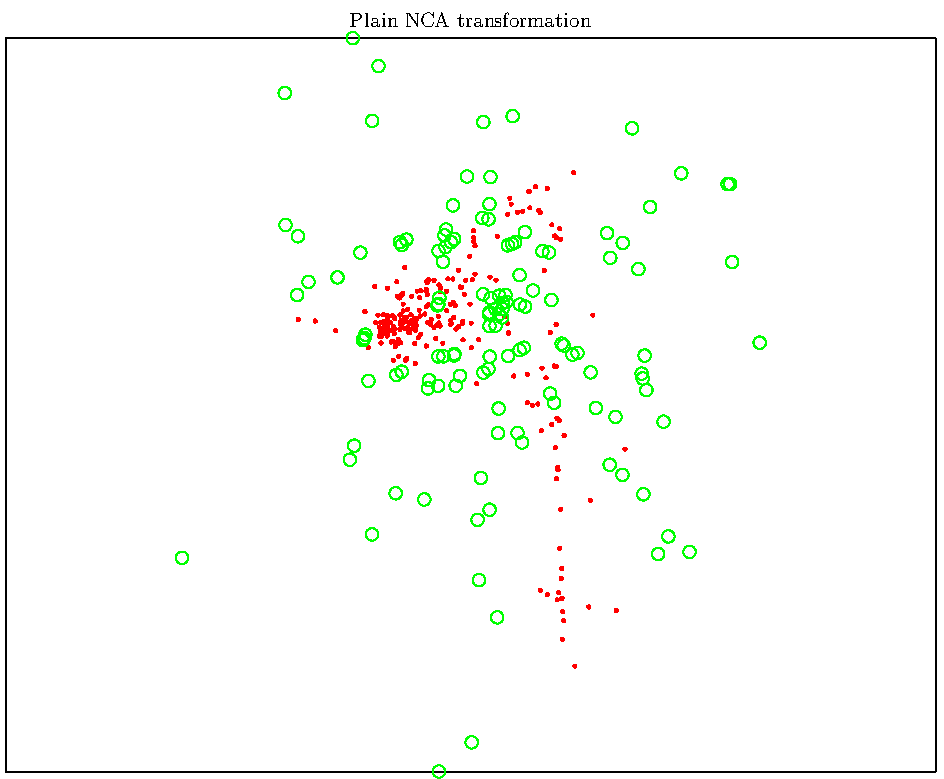
\includegraphics[width=0.45\textwidth]{images/sa-1}}
			    \hspace{0.02\textwidth}
			 \subfigure[NCA with dimensionality annealing projection]{\label{fig:sa-2}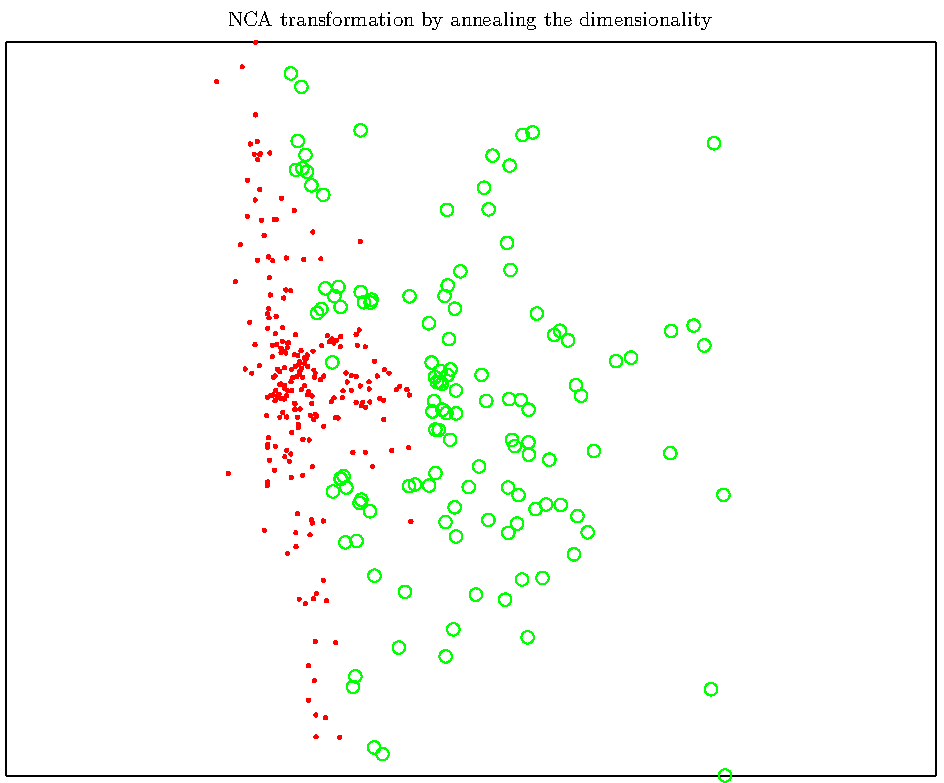
\includegraphics[width=0.45\textwidth]{images/sa-2}}
		\caption{Example of applying the dimensionality annealing procedure to \texttt{ionosphere} data set. The method using dimensionality annealing is more visually appealing than the classical approach.}
		\label{fig:simulated-annealing}
	\end{figure}
